\subsection{Fantasia3D}\label{fantasia3D}

The model proposed by \citeauthor{chen2023fantasia3d} takes a different approach in generating 3D Models from text inputs. It stands out for its approach to disentangling geometry and appearance in the generated 3D models, thereby achieving higher quality and more detailed rendering compared to NeRFs\@. Conventional NeRF uses volume rendering which combines the learning of the surface geometry with that of pixel colors, which makes them less effective for surface recovery. This approach does not allow for tracting the surface of an object and thus lacks in tuning detailed material and texture. Fantasia3D can result in more realisitc outputs using the hybrit scene representation of DMTet, ``which maintains a deformable tetrahedral grid and a differentiable mesh extraction layer; deformation can thus be learned through the layer to explicitly control the shape generation'' \citep{chen2023fantasia3d}.

\begin{figure}[ht]
    \centering
      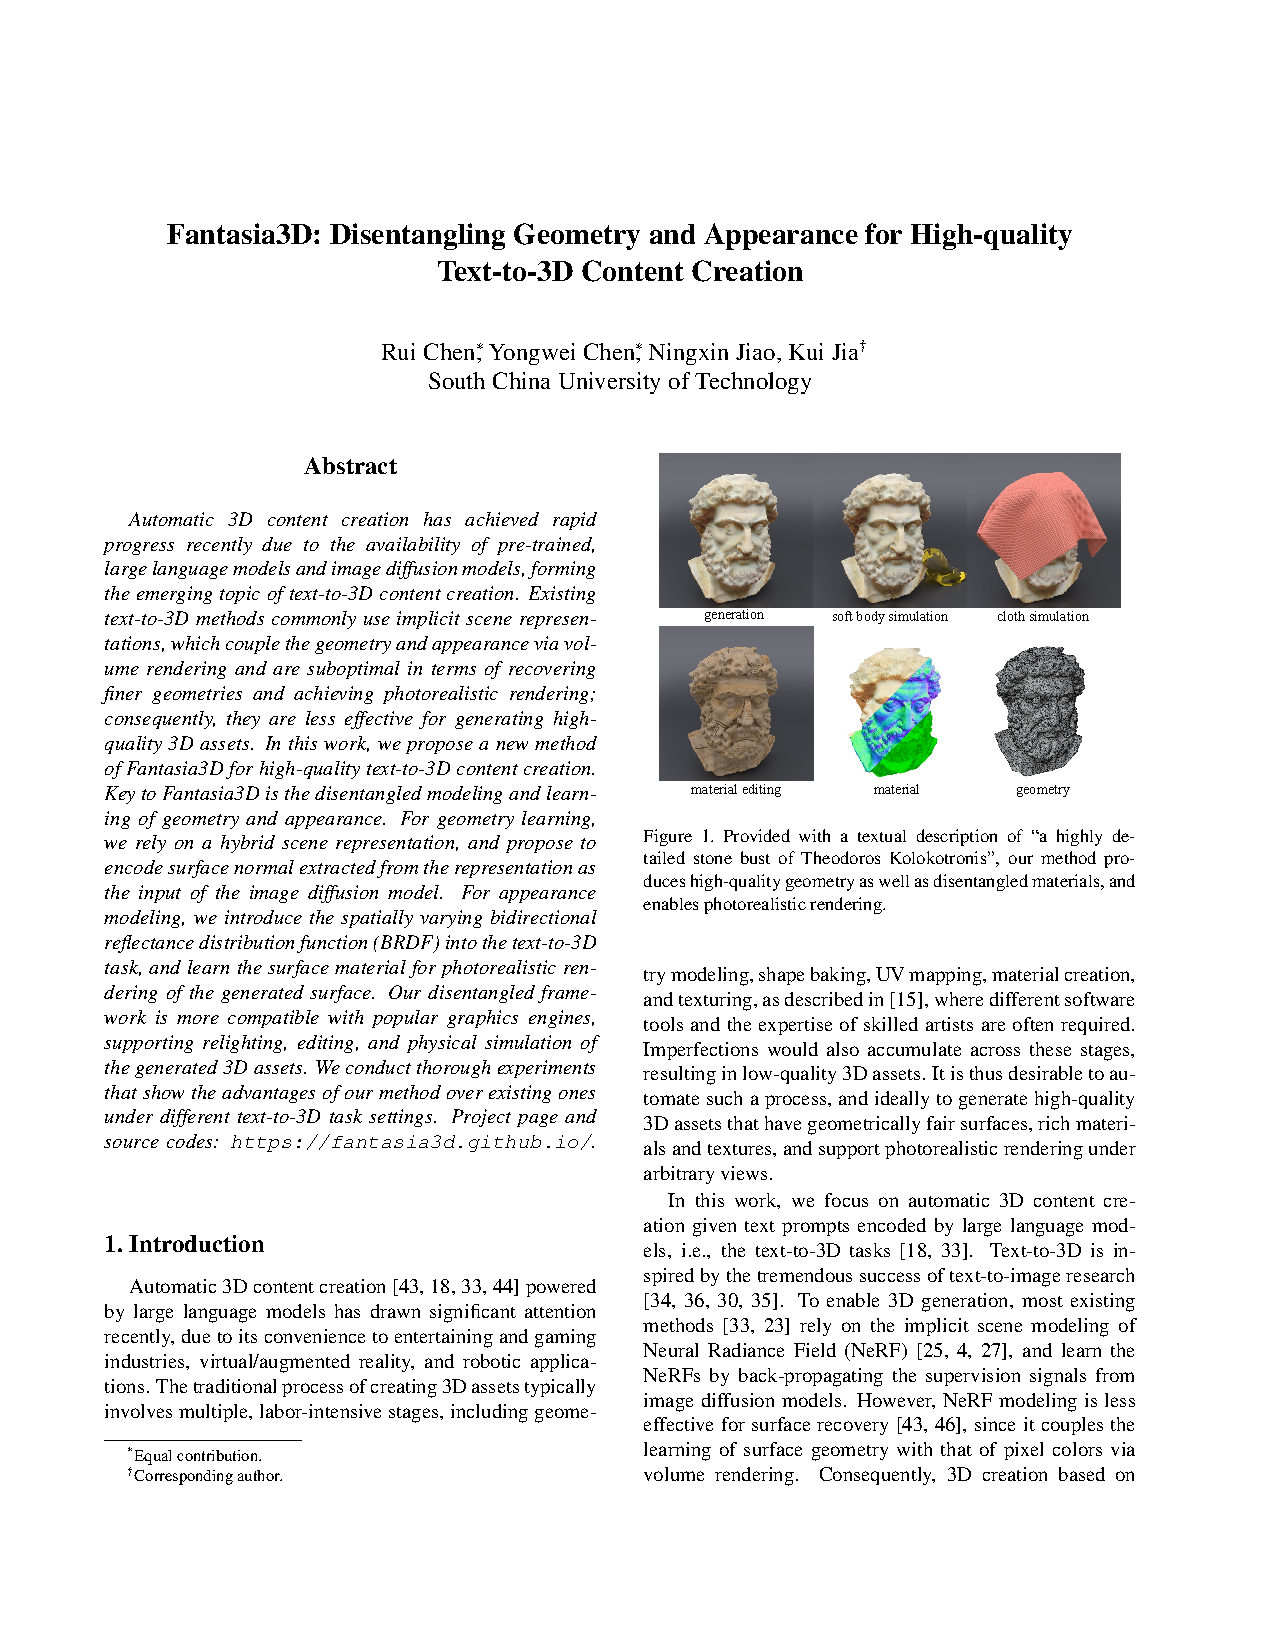
\includegraphics[width=1\columnwidth]{figures/Fantasia3D.png}
      \caption{Outline of the method Fantasia3D. Figure taken From \citep{chen2023fantasia3d}}\label{fig:figureFantasia}
\end{figure}

The geometry stage of Fantasia3D releis on a DMTet which paramererizes the 3D geometry as an MLP\@. 
In the first steps of geometry modeling, Fantasia3D renders and encodes surface normals and the object masks extracted from DMTet, while in the later stages only the rendered normal map is used for the shape encoding \citep{chen2023fantasia3d}. The default initialisation of the DMTet is an ellipsoid, while the model also accepts custom input allowing for more flexibility.  


Appearance Modeling trains another MLP which applies Bidirectional Reflectance Distribution Function (BRDF) on a learned DMTet, ``that predicts parameters of surface material and supports high-qualits 3D generation via photorealistic rendering'' \citep{chen2023fantasia3d}. This function uses the diffuse value \(\text{k}_d\), roughness and metallic \(\text{k}_{rm}\) and normal variation \(\text{k}_n\) in order to apply shading to the geometry. Then, an image is rendered along every ray and the loss is determined using SDS in order tu update the models parameters.    


Both geometry and appearance MLPs are learned through a pre-trained stable diffusion model \citep{rombachStableDiffusion} using Score Distillation Sampling (SDS) loss. 


Fantasia3D allows additional user inputs such as customized 3D shapes or generic 3D shapes of specific categories. This flexibility enhances user control over the content generation process. The disentangled generation of geometry and appearance makes the method compatible with popular graphics engines, supporting relighting, editing, and physical simulation of the generated 3D assets.

While Fantasia3D shows promise in generating photorealistic 3D assets from text, it faces challenges in generating loose geometries like hair, fur, and grass. Additionally, it primarily focuses on object generation, lacking the capacity to create complete scenes with backgrounds from text prompts. Future research aims to address these limitations.
